\documentclass{beamer}
\usetheme{Madrid}
\usecolortheme{beaver}
\usepackage{graphicx}
\usepackage{color}
\usepackage{tikz}
\usetikzlibrary{calc,arrows.meta,positioning,shapes}
\usepackage[utf8]{inputenc}

\newcommand{\bi}{\begin{itemize}}
\newcommand{\ei}{\end{itemize}}

%Information to be included in the title page:
\title[Neural Networks]{String Theory meets Machine Learning\\
- Neural Networks}
\author[R. Schneider]{Robin Schneider}
\institute[Uppsala University]{Uppsala University}
\date[November 2020]{November 2020}



\begin{document}
	
	\frame{\titlepage}
	
\begin{frame}
\frametitle{What is machine learning?}

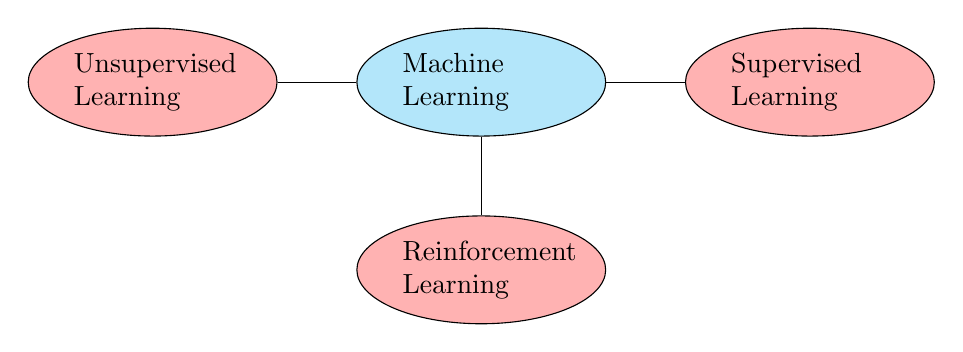
\begin{tikzpicture}
	\node[draw,fill=cyan!30,ellipse,text width=2cm] (1)
	{Machine Learning};
	\node[draw,fill=red!30,ellipse,text width=2cm] (2) [right =of 1]
	{Supervised Learning};
	\node[draw,fill=red!30,ellipse,text width=2cm] (3) [left =of 1]
{Unsupervised Learning};
	\node[draw,fill=red!30,ellipse,text width=2cm] (4) [below =of 1]
{Reinforcement Learning};	
	\draw (1) -- (2);
	\draw (1) -- (3);
	\draw (1) -- (4);
\end{tikzpicture}

\pause {\it It’s really just curve fitting, or ‘regression’, with a very, very large number of parameters.}

\qquad \qquad \qquad \qquad Jared Kaplan

\end{frame}

\begin{frame}
\frametitle{Why is ML useful for String theory?}
\begin{itemize}
	\item Universal Approximation theorem - A sufficient wide and deep NN can approximate almost any function we are interested in.
	\item \pause Computations are (NP) hard {\color{blue} [1809.08279]}.
	\bi \item Gröbner basis are double exponential
	\item Non linear Diophantine equations are undecidable
	 \ei 
	\item \pause Computations are plenty full.
	\bi \item Up to $10^{428}$ topological inequivalent CY 3-folds {\color{blue} [2008.01730]} %https://inspirehep.net/literature/1810205
	\item F-theory: $10^{272.000}$ flux vacua {\color{blue} [1511.03209]}%https://arxiv.org/abs/1511.03209
	\ei 
\end{itemize}

\end{frame}

\begin{frame}
\frametitle{Overview - Five Sessions}
\begin{enumerate}
	\item Neural Networks and Experiments
	\bi \item Learning stability and Hodge numbers. \ei
	\item Regularization and Convolutional Neural Networks
	\bi \item Learning more Hodge numbers. \ei
	\item Hyperparameter optimization
	\bi \item Learning Ricci flat metrics \ei
	\item (Variational) Autoencoder
	\bi \item Clustering of standard like models \ei
	\item Reinforcement learning
	\bi \item Exploring standard like models \ei
\end{enumerate}
\end{frame}

\begin{frame}
\frametitle{Literature}
Physics:
\begin{itemize}
	\item Fabian Ruehle - Data science applications to string theory
	\item Jared Kaplan - Notes on Contemporary Machine Learning for Physicists
	\item Pankaj Mehta et al. - A high-bias, low-variance introduction to Machine Learning for physicists
\ei
\pause 
Machine Learning:
\bi	
	\item Christoper M. Bishop - Pattern Recognition and Machine Learning
	\item Ian Goodfellow and Yoshua Bengio and Aaron Courville - Deep Learning
\end{itemize}
\end{frame}


\begin{frame}
\frametitle{Notation and Statistics}
\textbf{Probability Distributions}
\begin{itemize}
	\item likelihood function $p(D| \theta)$, observing data $D$, given parameters $\theta$.
	\item joint probability distribution $p(D, \theta) = p(D| \theta) p(\theta)$.
	\item prior $p(\theta)$ belief %and marginal distribution $p(D) = \sum_\theta p(D,\theta)$
	\item posterior distribution $p(\theta | D)$, having parameters $\theta$ given data $D$.
\end{itemize}
\pause \textbf{Central limit theorem} the sum of a set of random variables has a distribution that becomes increasingly Gaussian:
\begin{align}
\mathcal{N} (x|\mu, \sigma^2) = \frac{1}{\sqrt{2 \pi \sigma^2}} \exp \left[ - \frac{1}{2 \sigma^2} (x-\mu)^2 \right]
\end{align}
\end{frame}


\begin{frame}
\frametitle{Bayesian Inference and MLE}
\textbf{Sum and Product rule}
\begin{align}
\underbrace{p(D) = \sum_\theta p(D, \theta)}_{\text{sum rule}} \rightarrow \int p(D,\theta) d\theta = \int \underbrace{p(D|\theta) p(\theta)}_{\text{product rule}} d\theta = \mathbb{E}_\theta [p(D|\theta)]
\end{align}
\pause \textbf{Bayes theorem}
\begin{align}
p(\theta | D) = \frac{p(D|\theta) p(\theta)}{p(D)} =  \frac{p(D|\theta) p(\theta)}{\int d\theta' p(D|\theta') p(\theta')}
\end{align}
\pause \textbf{Maximum (Log) Likelihood Estimation}
\begin{align}
\hat{\theta} = \arg \underset{\theta}{\max} \log p(D|\theta)
\end{align}
\end{frame}


\begin{frame}
\frametitle{What is a Neural Network?}
	\begin{figure}[t]
		\centering
		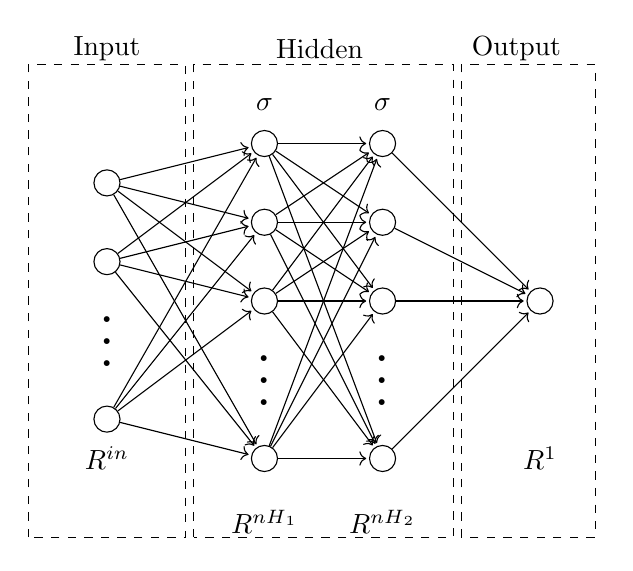
\begin{tikzpicture}[shorten >=1pt,node distance=2cm,auto]
		\tikzset{
			annot/.style={
				text width=4em,
				text centered,		
			}
		}
		\tikzset{%
			every neuron/.style={
				circle,
				draw,
			},
			neuron missing/.style={
				draw=none, 
				scale=2,
				text height=0.333cm,
				execute at begin node=\color{black}$\vdots$
			},
		}
		
		% Frames
		\draw[dashed] (0,0) rectangle (2,6);
		\draw[dashed] (2.1,0) rectangle (5.4,6);
		\draw[dashed] (5.5,0) rectangle (7.2,6);
		
		% Neuron Nodes
		% Input
		\foreach \m/\l [count=\y] in {1,2,missing,4}
		\node [every neuron/.try, neuron \m/.try] (I-\m) at (1,5.5-\y) {};%
		\node [annot] (Input) at (1,6.2) {Input};%
		\node [annot] (IR) at (1,1) {$\mathbb{R}^{in}$};%

		%H1
		\foreach \m/\l [count=\y] in {1,2,3,missing,4}
		\node [every neuron/.try, neuron \m/.try] (H1-\m) at (3,6-\y) {};
		\node [annot] (H1a) at (3,5.5) {$\sigma$};%
		\node [annot] (H1R) at (3,0.2) {$\mathbb{R}^{\text{nH}_1}$};%
		
		%H2
		\foreach \m/\l [count=\y] in {1,2,3,missing,4}
		\node [every neuron/.try, neuron \m/.try] (H2-\m) at (4.5,6-\y) {};%
		\node [annot] (H2a) at (4.5,5.5) {$\sigma$};%
		\node [annot] (H2R) at (4.5,0.2) {$\mathbb{R}^{\text{nH}_2}$};%
		\node [annot] (Hidden) at (3.7,6.2) {Hidden};	
		
		%O1
		\foreach \m/\l [count=\y] in {1}
		\node [every neuron/.try, neuron \m/.try] (O1-\m) at (6.5,4-\y) {};%
		\node [annot] (O2R) at (6.5,1) {$\mathbb{R}^{1}$};%
		%\node [annot] (O2l) at (11.5,6) {Value};%
		\node [annot] (Output) at (6.2,6.2) {Output};		
		
		% Connecting lines
		\foreach \i in {1,2,4}
		\foreach \j in {1,...,4}
		\draw [->] (I-\i) -- (H1-\j);
		\foreach \i in {1,...,4}
		\foreach \j in {1,...,4}
		\draw [->] (H1-\i) -- (H2-\j);
		\foreach \i in {1,...,4}
		\foreach \j in {1}
		\draw [->] (H2-\i) -- (O1-\j);
		\end{tikzpicture}
	\caption{\it A fully connected Neural Network of a regression problem.}
	\label{NNreg}
\end{figure}

\end{frame}


\begin{frame}
\frametitle{What is a Neural Network?}
\begin{figure}[t]
	\centering
	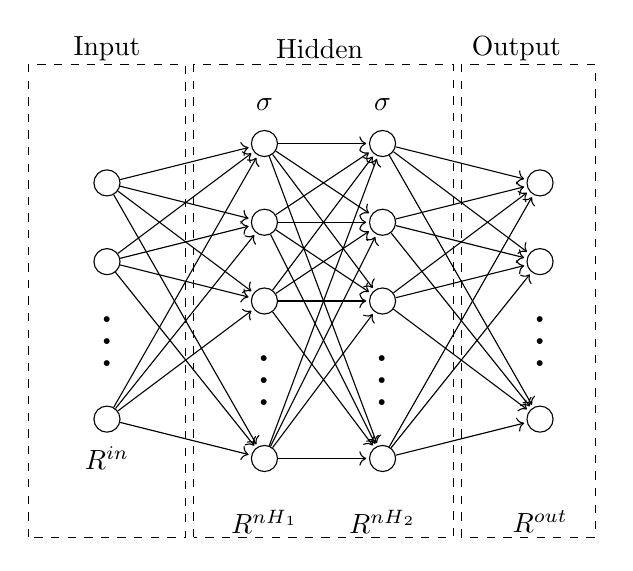
\begin{tikzpicture}[shorten >=1pt,node distance=2cm,auto]
	\tikzset{
		annot/.style={
			text width=4em,
			text centered,		
		}
	}
	\tikzset{%
		every neuron/.style={
			circle,
			draw,
		},
		neuron missing/.style={
			draw=none, 
			scale=2,
			text height=0.333cm,
			execute at begin node=\color{black}$\vdots$
		},
	}
	
	% Frames
	\draw[dashed] (0,0) rectangle (2,6);
	\draw[dashed] (2.1,0) rectangle (5.4,6);
	\draw[dashed] (5.5,0) rectangle (7.2,6);
	
	% Neuron Nodes
	% Input
	\foreach \m/\l [count=\y] in {1,2,missing,4}
	\node [every neuron/.try, neuron \m/.try] (I-\m) at (1,5.5-\y) {};%
	\node [annot] (Input) at (1,6.2) {Input};%
	\node [annot] (IR) at (1,1) {$\mathbb{R}^{in}$};%
	
	%H1
	\foreach \m/\l [count=\y] in {1,2,3,missing,4}
	\node [every neuron/.try, neuron \m/.try] (H1-\m) at (3,6-\y) {};
	\node [annot] (H1a) at (3,5.5) {$\sigma$};%
	\node [annot] (H1R) at (3,0.2) {$\mathbb{R}^{\text{nH}_1}$};%
	
	%H2
	\foreach \m/\l [count=\y] in {1,2,3,missing,4}
	\node [every neuron/.try, neuron \m/.try] (H2-\m) at (4.5,6-\y) {};%
	\node [annot] (H2a) at (4.5,5.5) {$\sigma$};%
	\node [annot] (H2R) at (4.5,0.2) {$\mathbb{R}^{\text{nH}_2}$};%
	\node [annot] (Hidden) at (3.7,6.2) {Hidden};	
	
	%O1
	\foreach \m/\l [count=\y] in {1,2,missing,4}
	\node [every neuron/.try, neuron \m/.try] (O1-\m) at (6.5,5.5-\y) {};%
	\node [annot] (O2R) at (6.5,0.2) {$\mathbb{R}^{out}$};%
	%\node [annot] (O2l) at (11.5,6) {Value};%
	\node [annot] (Output) at (6.2,6.2) {Output};		
	
	% Connecting lines
	\foreach \i in {1,2,4}
	\foreach \j in {1,...,4}
	\draw [->] (I-\i) -- (H1-\j);
	\foreach \i in {1,...,4}
	\foreach \j in {1,...,4}
	\draw [->] (H1-\i) -- (H2-\j);
	\foreach \i in {1,...,4}
	\foreach \j in {1,2,4}
	\draw [->] (H2-\i) -- (O1-\j);
	\end{tikzpicture}
	\caption{\it A fully connected Neural Network of a classification problem.}
	\label{NNclass}
\end{figure}
\end{frame}

\begin{frame}
\frametitle{A Neural Network}
We have a map $f(x;\{W,b\}) \simeq p(y|x,W,b)$:
\begin{align}
	f: \mathbb{R}^{in} \rightarrow \begin{cases}
	\mathbb{R}^{1} &\text{ regression }\\
	\mathbb{R}^{out} &\text{ classification }
	\end{cases}
\end{align}
at each hidden layer we have
\begin{align}
	&H_1: a_1 = \sigma_1 ( z_1 = W_1 x + b_1) \\
	& \qquad \qquad \vdots \nonumber
	%&H_2: z_2 = \sigma_2 ( W_2 z_1 + b_2)  
\end{align}
and at the output
\begin{align}
out = 
	\begin{cases}
	W_n a_{n-1} + b_{n}, \quad &\text{regression} \\
	\text{softmax}(W_n a_{n-1} + b_{n}) \quad &\text{classification}
	\end{cases}
\end{align}
\end{frame}

\begin{frame}
\frametitle{Activation Functions}
\begin{figure}[t]
	
	\centering
	\begin{minipage}{0.3\linewidth}
		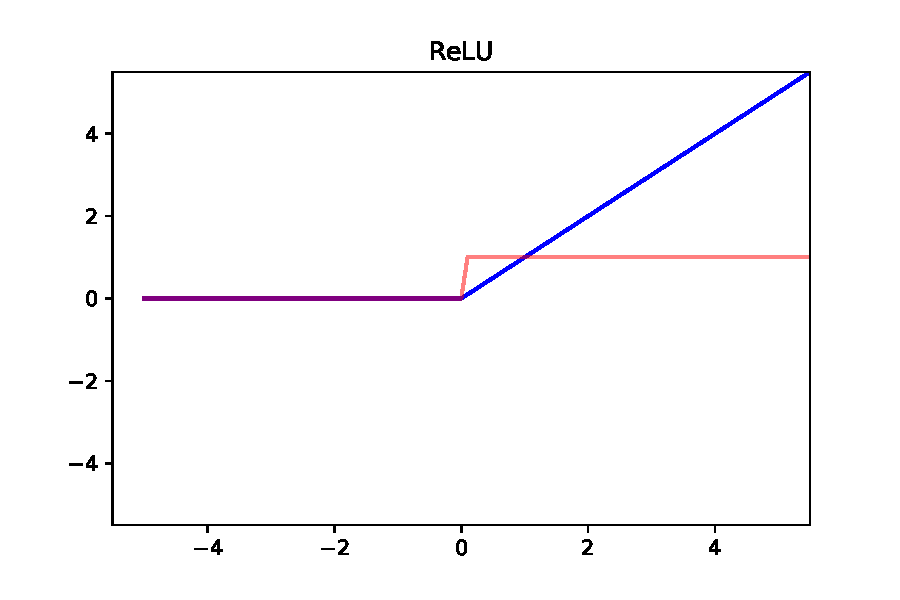
\includegraphics[scale=0.27]{relu.pdf}
	\end{minipage}
	\begin{minipage}{0.3\linewidth}
		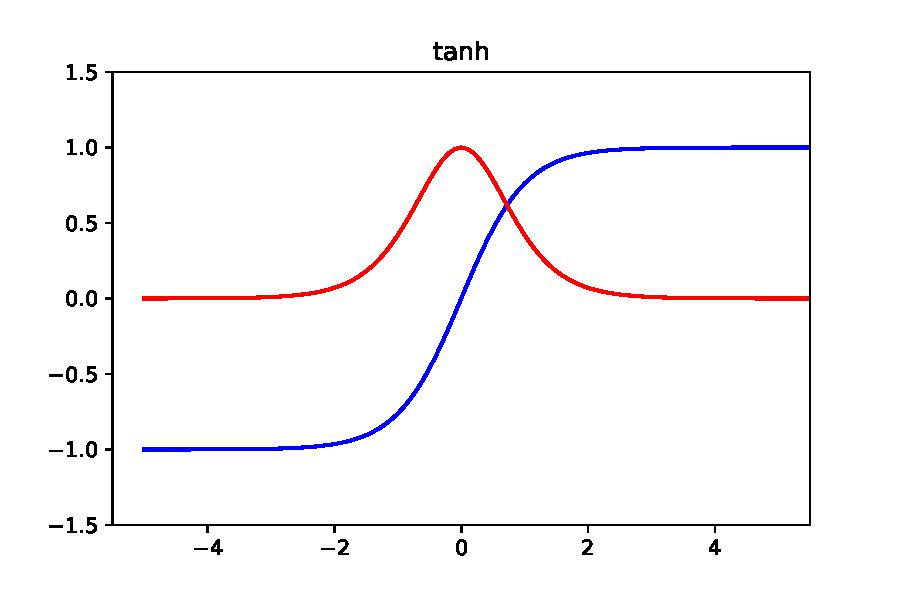
\includegraphics[scale=0.27]{tanh.pdf}
	\end{minipage}
	\begin{minipage}{0.3\linewidth}
		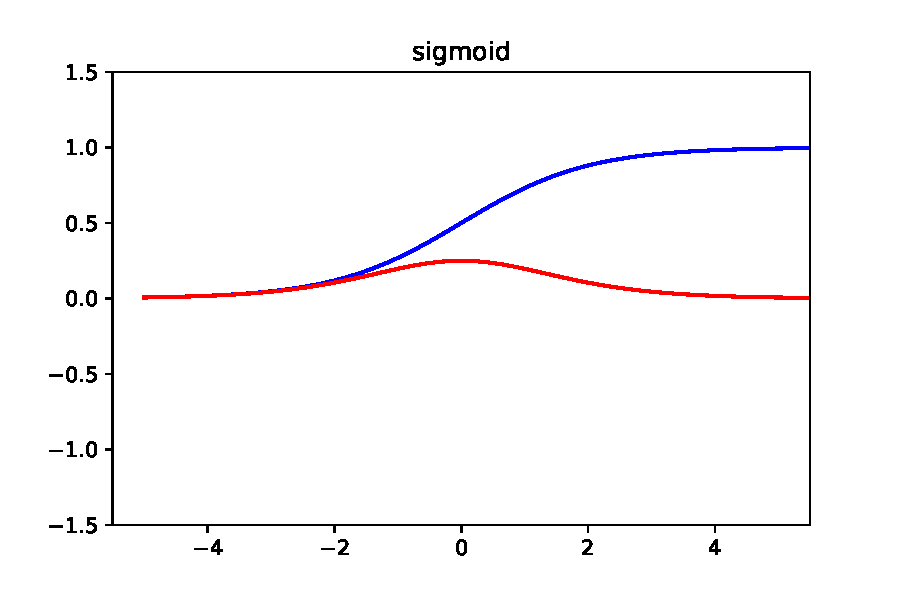
\includegraphics[scale=0.27]{sigmoid.pdf}
	\end{minipage}
	\caption{\it ReLU, tanh and sigmoid function in blue, their derivatives in red.}
	\label{fig:act}
\end{figure}

Typically we have, ReLU, tanh or sigmoid:
\begin{align}
	\sigma(x) = \begin{cases}
	x \quad \text{if } x>0\\
	0 \quad \text{if } x<0
	\end{cases},
	\qquad \sigma (x) = \tanh (x), \qquad \sigma (x) = \frac{1}{1 + e^{-x}}.
\end{align}
\end{frame}

\begin{frame}
\frametitle{Optimization and loss function}
We optimize with respect to some objective $J$. Take a classical regression problem, i.e. curve fitting with just one layer
\begin{align}
	J = \frac{1}{2} \sum_i (y_i - f(x_i; \theta))^2
\end{align}
is just least square. Generally we denote NN parameters as $\theta = \{ W_1, b_1, \dots \}$.\\
\vspace{0.5cm}
\pause 
Parameter space of NN is non convex, which makes rigorous mathematical results more tricky.

Nevertheless, we can motivate least square with maximum likelihood estimation. Assume NN consisting of a single layer, i.e. simple regression.
\end{frame}

\begin{frame}
\frametitle{Maximum Likelihood Estimator}
Start from a Gaussian
\begin{align}
\label{normal}
p(y_i|x_i,\theta) = \mathcal{N}(y_i|\mu(x_i), \sigma^2(x_i)) % = \frac{1}{\sqrt{2 \pi \sigma^2}} \exp \left[ - \frac{1}{2 \sigma^2} (x-\mu)^2 \right]
\end{align}
the MLE tells us for some data 
\begin{align}
	\hat{\theta} = \arg \underset{\theta}{\max} \log p(y_i|x_i,\theta)
\end{align}
assume samples are independent and identically distributed
\begin{align}
	p(y|x,\theta) = \Pi_{i=1}^n \mathcal{N}(y_i|\mu(x_i), \sigma^2(x_i))
\end{align}
\pause
we find the log likelihood
\begin{align}
	l(\theta) &= \log p(y|x,\theta) = \sum_{i=1}^{n} \log p(y_i|x_i, \theta) \nonumber \\
	& \stackrel{\ref{normal}}{=} -\frac{1}{2 \sigma^2} \sum_i^n (y_i -  \underbrace{\theta x_i}_{f(x_i; \theta)})^2 - \frac{n}{2} \log (2 \pi \sigma^2)
\end{align}
where we used $\mu = \theta x$ and some fixed variance $\sigma(x)^2 = \sigma^2$.
\end{frame}

\begin{frame}
\frametitle{Stochastic Gradient Descent}
\textbf{Stochastic} - we use (mini)batches.

\textbf{Gradient descent}, we compute the direction towards the next minimum w.r.t. the weights
\begin{align}
	g^k_\theta = \nabla_\theta J
\end{align}
and then update the weights
\begin{align}
	\theta_{k+1} = \theta_k - \epsilon g^k_\theta
\end{align}
where $\epsilon$ is called the learning rate. 
\pause

\textbf{Momentum}
\begin{align}
g^k_\theta =  \nabla_\theta J - \alpha g^{k-1}_\theta
\end{align}
\end{frame}

\begin{frame}
\frametitle{Backpropagation I}
How to optimize in practice? Compute derivatives
\begin{align}
	\partial_\theta J &= \sum_i^{\text{nB}} \partial_\theta J(x_i, \theta) \nonumber \\
	& = \sum_i^{\text{nB}} (y_i - f(x_i, \theta)) \partial_\theta f(x_i, \theta) \nonumber  \\
	& = \sum_i^{\text{nB}} (y_i - f(x_i, \theta)) x_i 
\end{align}
\pause
Consider more layers
\begin{align}
	& = \sum_i^{\text{nB}} (y_i - f(x_i, \theta)) \partial_\theta a_{n-1} \nonumber \\
	& = \sum_i^{\text{nB}} (y_i - f(x_i, \theta)) \sigma'(z_{n-1}) \partial_\theta z_{n-1} = \qquad  \hdots 
\end{align}

\end{frame}

\begin{frame}
\frametitle{Backpropagation II}
This brings us to backpropagation. We compute chain rule of each part, save results and multiply them together. Typical derivatives of activation functions
\begin{align}
	&\partial_x \text{Relu}(x) = \begin{cases}
	1 \text{ if } x>0\\
	0 \text{ else}
	\end{cases} \\
	&\partial_x \tanh(x) = 1 - \tanh^2(x) \\
	&\partial_x \text{sigmoid}(x) = \text{sigmoid}(x) (1 - \text{sigmoid}(x))
\end{align}

\end{frame}

\begin{frame}
\frametitle{Classification}
Take only two classes with {\it cross entropy} as loss function
\begin{align}
	J & = \frac{1}{n} \sum_i H(p(x_i),q(x_i)) \text{ with } H(p,q) = - \sum_j p_j(x) \log (q_j(x)) 
\end{align}	
where $p_j(x)$ are the discrete true labels and $q_j(x)$ the predictions.
Consider logistic
\begin{align}
q_{y=1} = \sigma (x; \theta)= \frac{1}{1 + e^{-\theta x}} \; \text{ and } \; q_{y=0} = 1- q_{y=1}
\end{align}
Then rewrite cross entropy as average over data points
\begin{align}
	&J = - \frac{1}{n} \sum_i y_i \log ( \sigma (x_i; \theta)) + (1-y_i) \log( 1 - \sigma (x_i; \theta)).
\end{align}

\end{frame}

\begin{frame}
\frametitle{MLE}
Likelihood of observing data $D = (x_i, y_i)$ is
\begin{align}
P(D|\theta) = \Pi_i^{n} \sigma( x_i; \theta)^{y_i} (1 - \sigma( x_i; \theta))^{1-y_i}
\end{align}
Thus the log likelihood becomes
\begin{align}
l(\theta) = \sum_{i=1}^n y_i \log (\sigma(x_i; \theta)) + (1-y_i) \log( 1 - \sigma(x_i; \theta))
\end{align}
\pause
Compute gradient for backpropagation
\begin{align}
	&\partial_x \text{sigmoid}(x) = \text{sigmoid}(x) (1 - \text{sigmoid}(x))
\end{align}
such that
\begin{align}
	\partial_\theta J = \sum_{i=1} x_i (y_i - \sigma(x_i; \theta)) 
\end{align}
\end{frame}

\begin{frame}
\frametitle{More Classes and Layers - Softmax}
One hot encoding. Treat $N$ classes as vector $y_j \in \mathbb{Z}^N$ with all 0 except of a single 1. Use softmax activation function in last layer:
\begin{align}
p_j(y|x ; \theta) = \frac{e^{a_j}}{\sum_k^N e^{a_k}}
\end{align}
which has derivatives
\begin{align}
	\frac{\partial p_j(a)}{\partial a_k} = 
	p_j(a) ( \delta_{jk}- p_k(a)) .
\end{align}
\pause
Again take crossentropy as a loss function
\begin{align}
J = - \frac{1}{n} \sum_{i=1}^n \sum_{j=1}^N  y_{ij} \log (p_j(x_i; \theta))
	%J = - \sum_{i=1}^n \sum_{j=1}^N  y_{ij} \log (\sigma(x_i; \theta)) + (1-y_{i,j}) \log( 1 - \sigma(x_i; \theta))
\end{align}
we take derivatives and find
\begin{align}
	\frac{\partial J}{\partial a_j} = \frac{1}{n} \sum_{i} p_j(a_i) - y_{ij}.
\end{align}
\end{frame}

\begin{frame}
\frametitle{Experiment set up}
How to conduct a ML experiment.
\begin{enumerate}
	\item Define the problem
	\pause
	\item Create some data
	\pause
	\item Make a train test split
	\pause
	\item Run many experiments with different NNs
	\pause
	\item Repeat
	\item (Profit)
\end{enumerate}
\end{frame}


\begin{frame}
\frametitle{Application: Learning Stability}
Reproduce some results of the early literature
\begin{itemize}
	\item F. Ruehle - {\it Evolving neural networks with genetic algorithms to study the String Landscape}
	\item We will predict stability of line bundles over a CY manifolds using a fully connected NN.
	\item We will implement the fully connected NN from scratch.
\end{itemize}
\end{frame}

\begin{frame}
\frametitle{Application: Learning Stability}
Consider the following Complete Intersection Calabi Yau (bicubic):
\begin{align}
M = \left[
\begin{array}{c||c}
2 & 3\\
2 & 3
\end{array}
\right]
\end{align}
The slope of a line bundle over it is given by
\begin{align}
\mu(L) = d_{ijk} q^i t^j t^k = 6q_0t_0t_1 + 3q_0t_1^2 + 3q_1t_0^2 + 6q_1t_0t_1
\end{align}
a line bundle is slope stable iff
\begin{align}
	\mu(L) = 0\qquad \forall t^j > 0
\end{align}
somewhere in the Kähler cone.
\end{frame}

\end{document}